% -*- TeX:UTF-8 -*-
%%
%% KAIST 학위논문양식 LaTeX용 (ver 0.5)
%%

\documentclass[master,english,final]{kaist-ucs}

% 추가 패키지
\usepackage{amsmath, amssymb}
\usepackage{booktabs}

% @command title 논문 제목
\title[korean] {관상동맥 파열위험지표 정의 및 민감도 분석}
\title[english]{Definition of a Coronary Plaque Rupture Risk Index and Its Sensitivity Analysis}

% @command author 저자 이름
\author[korean]{김}{세 혁}
\author[korean2]{김}{세혁}
\author[chinese]{金}{世 赫}
\author[english]{Kim}{Sehyeog}

% @command advisor 지도교수 이름
\advisor[major]{김 현 진}{Hyun Jin Kim}{signed}
\advisor[major2]{김현진}{Hyun Jin Kim}{signed}
\advisorinfo{Professor of Mechanical Engineering}

% @command department
\department{ME}{engineering}{c}

% @command referee 심사위원
\referee[1]{김 현 진}
\referee[2]{유 승 화}
\referee[3]{이 익 진}

\approvaldate{2026}{05}{27}
\refereedate{2026}{05}{27}
\gradyear{2026}

% 본문 시작
\begin{document}

\thesisinfo

%% 한글 초록: 500자 미만
\begin{summary}
관상동맥 플라크 파열은 급성 관상동맥 증후군의 주된 원인이며 형태, 혈류역학, 재료 세 인자군이 복합적으로 작용한다. 
완전 연성 맥동 유체-고체 연성 해석의 높은 계산 비용으로 인해 세 인자군을 동시에 대규모로 다룬 연구는 부재하였다. 
본 학위논문은 첫째, 맥동 하중의 시간 성분과 공간 성분을 분리하여 완전 연성 해석 대비 30배 이상의 비용 절감과 최대 4.5\% 수준의 
응력 오차를 달성하는 비용효율적 유체-고체 연성 해석 기법을 제안하고 검증하였다.
둘째, 위 방법을 사용하여 저감쇠 플라크와 석회화 플라크의 대규모 라틴 하이퍼큐브 데이터셋을 구축하고, 
응력과 강도의 비로 정의한 여섯 개 취약성 지수를 임상 일곱 기준으로 선별하였으며, 가우시안 과정 회귀 대리모델과 소볼 전역 민감도 분석으로 세 인자군의 기여를 정량화하였다. 
결과적으로 맥동 응력 진폭에 강도 정규화를 결합한 두 지수만이 임상적으로 일관되며, 재료물성이 파열 위험의 지배 인자군임을 규명하였다.
\end{summary}

\begin{Korkeyword}
관상동맥 플라크 파열, 유체-고체 연성 해석, 취약성 지수, 전역 민감도 분석, 가우시안 과정 회귀, 섬유막 강성
\end{Korkeyword}

%% 영문 초록: 300단어 미만
\begin{abstract}


\end{abstract}

\begin{Engkeyword}
Coronary plaque rupture is the leading cause of acute coronary syndrome, arising from the combined action of three factor groups: morphology, hemodynamics, and material properties. Because of the high computational cost of fully coupled pulsatile fluid–structure interaction (FSI) analysis, no prior study has addressed all three factor groups simultaneously at large scale.This thesis makes two contributions. First, it proposes and validates a cost-effective FSI scheme that decouples the temporal and spatial components of pulsatile loading, achieving more than a 30-fold reduction in computational cost relative to fully coupled FSI while keeping the maximum stress error within 4.5\%. 
Second, using this scheme, large-scale Latin Hypercube datasets are constructed for low-attenuation and calcified plaques; six vulnerability indices, defined as stress-to-strength ratios, are screened against seven clinical criteria; and the contributions of the three factor groups are quantified using Gaussian process regression surrogate models together with Sobol global sensitivity analysis. The results show that only two indices—those combining pulsatile stress amplitude with strength normalization—are clinically consistent, and material properties are identified as the dominant factor group governing rupture risk.\end{Engkeyword}

\addtocounter{pagemarker}{1}
\newpage

\tableofcontents
\listoftables
\listoffigures


%%======================================================================
%% Chapter 1. Introduction
%%======================================================================
\chapter{Introduction}

\section{Plaque rupture definition}
관상동맥(coronary artery)은 심장 근육에 혈액을 공급하는 혈관으로, 내막에 지질핵(lipid core), 섬유조직, 석회화 등이 축적되어 형성된 병변을 죽상경화성 플라크(atherosclerotic plaque)라 한다~\cite{bentzon2014, otsuka2016}. 플라크는 혈액이 지나는 내강(lumen)을 좁혀 심근으로 가는 혈류를 감소시키고, 이는 심근 허혈(myocardial ischemia)로 이어지며~\cite{bentzon2014}, 실제로 허혈성 심장질환은 전 세계 단일 사망원인 1위로, 연간 약 910만 명의 사망을 초래한 것으로 보고되었다~\cite{WHO2024Top10}.
플라크의 괴사핵과 내강 사이에는 둘을 분리하는 섬유막(fibrous cap)이 존재하며, 이 섬유막이 찢어지는 현상을 플라크 파열(plaque rupture)이라고 한다~\cite{virmani2000, otsuka2016}. 파열이 일어나면 혈전유발성(thrombogenic) 괴사핵이 혈류에 노출되어 혈소판 응집과 혈전(thrombus)이 급격히 형성되고 혈관이 폐색된다~\cite{otsuka2016}. 플라크 파열은 급성관상동맥증후군(acute coronary syndrome, ACS)의 주요 원인이며, 이로 인한 급성 심근경색(myocardial infarction)과 심혈관 사망으로 이어질 수 있다~\cite{lee2019, otsuka2016}.

\section{Causes}
임상적으로 플라크 파열은 생리학적·형태학적·혈류역학적 요인이 복합적으로 작용한 결과이다. 생리학적으로는 염증 반응, macrophage infiltration, extracellular matrix degradation, 석회화가, 형태학적으로는 얇은 섬유막, 큰 괴사핵, 협착률, plaque burden 등이 파열 취약성과 관련된다~\cite{bentzon2014, virmani2006}. 또한 wall shear stress, axial plaque stress, ΔFFR_CT등의 혈류역학적 지표는 형태학적 지표에 더해 급성 관상동맥 증후군의 원인 병변을 독립적으로 예측한다~\cite{lee2019emerald, yang2021hemodynamics}.
역학적으로 플라크 파열은 응력이 조직 강도를 초과할 때 발생하는 급성 사건이거나~\cite{choi2015aps, brown2016, gu2022}, 반복적인 혈압 하중에 의한 피로 파괴로 해석된다~\cite{bank2000, versluis2006}. 따라서 선행 연구들은 직접 모델링이 어려운 임상적 요인을 역학적 요인으로 환원하여, 생리학적 변화는 물성치와 강도로, 형태학적·혈류역학적 요인은 각각 응력 집중과 외부 하중으로 해석한다~\cite{brown2016, gu2022, corti2022}. 이에 본 연구도 파열 위험을 지배하는 역학적 요인을 물성치, 형태학적 특성, 혈류역학적 하중의 세 범주로 구분하여 분석하였다.

\section{Vulnerability indices}
플라크 파열 위험을 정량적으로 평가하기 위한 수치해석 연구는 주로 섬유막 응력에 기반하여 진행되어 왔으며, 이는 크게 정적 파괴(static failure)와 피로 파괴(fatigue failure)의 두 관점에서 해석될 수 있다. 정적 파괴 관점에서는 심박 주기 내에서 섬유막에 작용하는 최대 응력이 조직 강도를 초과할 때 파열이 발생한다고 보며, 이에 따라 수축기 최대 응력인 plaque structural stress (PSS)가 주요 지표로 사용되어 왔다~\cite{teng_pss, huang_pss}. 반면 피로 파괴 관점에서는 매 심박 주기마다 반복적으로 작용하는 하중에 의해 손상이 누적되어 파열이 발생한다고 보며~\cite{bank_fatigue_hypothesis, versluis_paris_fatigue}, 이 경우 파괴를 좌우하는 주요 인자는 최대응력 자체가 아니라 심박 주기 동안의 응력 변동폭, 즉 plaque structural stress variation ($\Delta$PSS)으로 해석된다~\cite{fatigue, costopoulos_vh_ivus}.
그러나 플라크의 취약성은 응력의 절대적인 크기만으로 결정되지 않는다. 동일한 응력이 작용하더라도 섬유막 강도가 낮은 경우 파열 위험은 더 크게 증가하며, 따라서 파열 위험은 응력이 섬유막 강도에 대해 얼마나 큰 상대적 수준을 갖는지로 평가되어야 한다~\cite{corti_vi}. 섬유막 강도는 콜라겐 함량과 미세구조 등 환자별 생리학적 특성에 의해 크게 달라지는 물성치로 알려져 있다~\cite{savvopoulos_collagen_modulus, chai_indentation}. 이에 따라 본 연구에서는 섬유막 강도를 $S_{fc}$로 정의하고, 정적 파괴와 피로 파괴를 함께 고려하기 위해 각각 $PSS/S_{fc}$와 $\Delta PSS/S_{fc}$를 vulnerability index로 사용하여 플라크 파열 위험을 분석한다.

\section{Limitations of prior parameteric computational studies}
플라크 파열 위험을 정량적으로 평가하기 위한 수치해석 연구는 주로 섬유막 응력에 기반하여 진행되어 왔으며, 이는 크게 정적 파괴(static failure)와 피로 파괴(fatigue failure)의 두 관점에서 해석될 수 있다. 정적 파괴 관점에서는 심박 주기 내에서 섬유막에 작용하는 최대 응력이 조직 강도를 초과할 때 파열이 발생한다고 보며, 이에 따라 수축기 최대 응력인 plaque structural stress (PSS)가 주요 지표로 사용되어 왔다~\cite{teng_pss, huang_pss}. 반면 피로 파괴 관점에서는 매 심박 주기마다 반복적으로 작용하는 하중에 의해 손상이 누적되어 파열이 발생한다고 보며~\cite{bank_fatigue_hypothesis, versluis_paris_fatigue}, 이 경우 파괴를 좌우하는 주요 인자는 최대응력 자체가 아니라 심박 주기 동안의 응력 변동폭, 즉 plaque structural stress variation ($\Delta$PSS)으로 해석된다~\cite{fatigue, costopoulos_vh_ivus}.
그러나 플라크의 취약성은 응력의 절대적인 크기만으로 결정되지 않는다. 동일한 응력이 작용하더라도 섬유막 강도가 낮은 경우 파열 위험은 더 크게 증가하며, 따라서 파열 위험은 응력이 섬유막 강도에 대해 얼마나 큰 상대적 수준을 갖는지로 평가되어야 한다~\cite{corti_vi}. 섬유막 강도는 콜라겐 함량과 미세구조 등 환자별 생리학적 특성에 의해 크게 달라지는 물성치로 알려져 있다~\cite{savvopoulos_collagen_modulus, chai_indentation}. 이에 따라 본 연구에서는 섬유막 강도를 $S_{fc}$로 정의하고, 정적 파괴와 피로 파괴를 함께 고려하기 위해 각각 $PSS/S_{fc}$와 $\Delta PSS/S_{fc}$를 vulnerability index로 사용하여 플라크 파열 위험을 분석한다.

\section{Present study}
본 연구는 선행연구들의 한계, 즉 세 인자군을 충분한 표본 수와 맥동성 하중 하에서 동시에 분석하지 못한 문제를, 서로 맞물리는 두 축으로 해소한다.
첫째 축 — 비용효율적 맥동성 FSI 기법의 개발과 검증 (Chapter 2). 
한계의 근본 원인인 완전 연성 맥동 FSI의 높은 계산 비용을 줄이기 위해, 맥동 하중의 시간 성분과 공간 성분을 분리하는 대안을 제시하고 검증한다. 이를 통해 대규모 표본에 대한 맥동 응력 해석을 현실적인 비용으로 수행할 수 있게 된다.
둘째 축 — 세 인자군 동시 대규모 맥동 민감도 분석 (Chapter 3~). 
첫째 축에서 확보한 forward solver를 기반으로, 파열 위험을 응력과 섬유막 강도의 비(VI = stress/strength)로 정의하며, stress(응력)으로 정적 파괴(PSS)와 피로 파괴(ΔPSS)를 함께 고려한다. 이후 형태·혈류역학·재료 세 인자군을 맥동 조건 하에서 동시에 변동시켜, 파열 위험지표에 대한 전역 민감도 분석(GSA)을 수행한다. 이로써 어느 인자군이 파열 위험을 지배하는지를 정량적으로 규명한다. 
두 축을 결합하여, 본 학위논문은 일관된 in-silico 파열 평가 프레임워크를 제시한다.



%%======================================================================
%% Chapter 2. Cost-effective FSI
%%======================================================================
\chapter{Cost-effective Fluid--Structure Interaction Method}

%2.1
\section{Framework}
본 기법의 핵심 아이디어는 맥동 하중의 **시간 성분과 공간 성분을 분리(decouple)**하는 것이다. 즉, 임의의 유체·고체 맥동 경계조건이 주어졌을 때 심장주기 내 목표 시점 t_a의 국소 혈관벽 응력장 σ(t_a)를, 단일 맥동 1차원(1D) 축소차수 해석(ROM)과 그 시점에서 평가한 정적(steady) 3차원 유체·구조 해석의 결합으로 근사한다. 이는 첨두 수축기나 이완기말과 같은 대표 시점의 생체역학 지표만으로도 충분한 진단 정보를 얻을 수 있다는 관찰에 근거하며, 시간 의존적 연성 문제 전체를 풀지 않고 대표 시점의 순간 응력 상태만을 추정한다.
여기서 ROM은 혈관을 축방향 1차원 네트워크로 축소하여 맥동 혈류를 저비용으로 푸는 모델로, 혈관 트리 전체에서 시간에 따른 압력·유량 파형을 계산한다. 다만 1D 축소만으로는 협착·분기처럼 기하가 복잡한 영역의 압력 손실을 충분히 포착하지 못하므로, 이러한 영역의 압력강하를 유량의 비선형 함수로 보정하는 물리 기반 항을 결합한다~\cite{choi2025rom}.

\begin{figure}[ht]
\centering
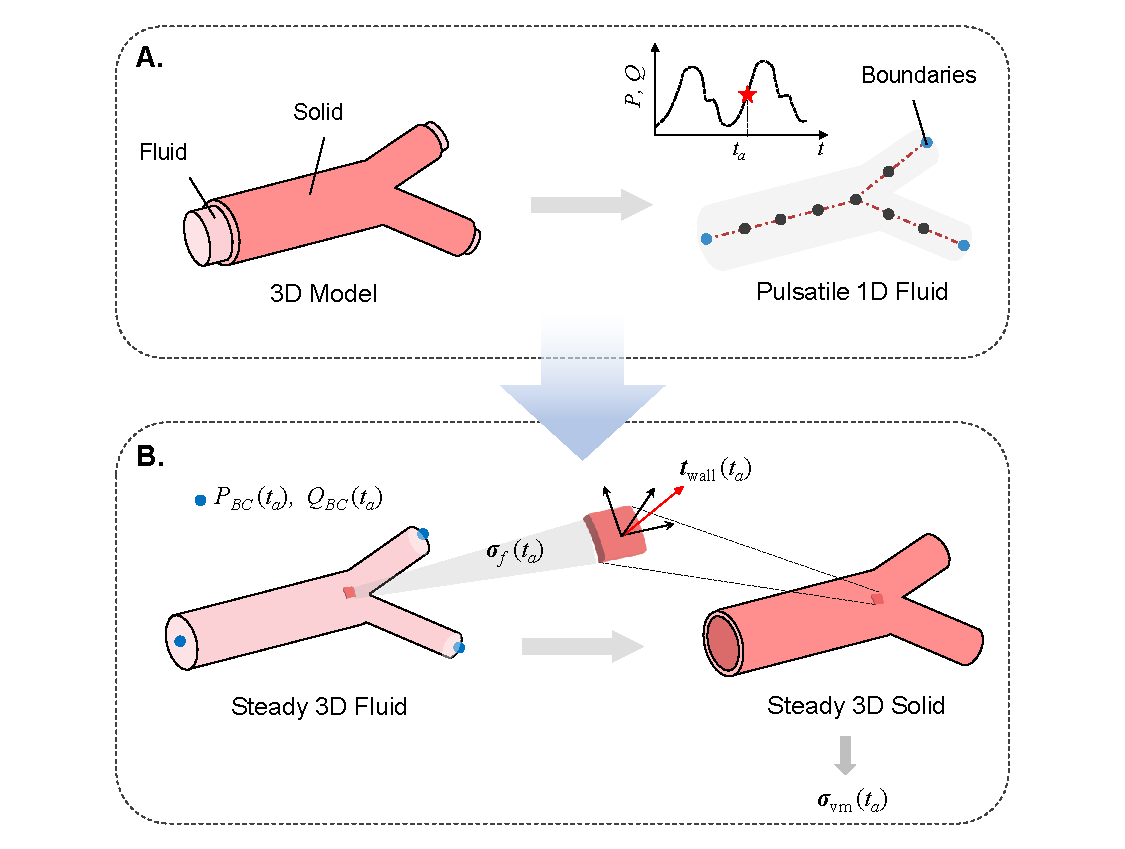
\includegraphics[width=0.95\textwidth]{figures/figure_page_01.pdf}
\caption[Cost-effective FSI framework]{Cost-effective FSI framework:snapshot-based coupling overview.}
\label{fig:cefsi-overview}
\end{figure}

Figure에서 구체적인 과정은 맥동 해석(Figure A)을 선행한 뒤 정적 해석(Figure B)으로 이어지며, 다음 세 단계로 구성된다. 

Step 1 (맥동 해석). 주어진 형상과 경계조건에 대해 물리 기반 1D 축소차수모델(ROM)로 맥동 해석을 수행하여 혈관 경계의 시간에 따른 압력·유량을 계산하고, 목표 시점 t_a에서의 값을 추출한다.
Step 2 (정적 해석). t_a의 경계조건으로 3D 유체 해석을 수행하여, 이후 응력 해석에 필요한 벽면 traction을 계산한다.
Step 3 (정적 해석). 이 traction을 부과한 3D 구조 해석으로 t_a에서의 응력장과 변위장을 도출한다.

즉, 비용이 큰 맥동 해석은 1D로 한 번만 수행해 연산 시간을 낮추고, 
원하는 각 목표 시점에 대해서는 Step 2–3을 3차원 정적 해석으로 반복함으로써 여러 시점의 응력장을 저비용으로 얻는다.

%2.2
\section{Governing Equations}
총 3가지 step 각각에 대해서, 지배방정식을 알아보고, 더하여 최종적으로 우리가 비교할 Full FSI 모델의 지배방정식까지 살펴보자.

\subsection{One-dimensional reduced-order hemodynamic (Step 1)}
\subsection{Three-dimensional steady fluid (Step 2)}
\subsection{Three-dimensional quasi-static structural problem (Step 3)}
\subsection{Reference fully coupled FSI formulation}



\section{Validaiton setup}
\subsection{Geometries and mesh}
제안 기법을 해부학적·혈류역학적 복잡도가 점증하는 세 가지 형상에 대해 검증하였다(Figure~\ref{fig:geo_ROMFSI}). 첫째, 이상적 좌전하행지(LAD) 관상동맥은 전체 길이 L=10~cm, lumen 반경 R=0.1~cm, 벽 두께 t=0.02~cm의 단순 원통 분절로, 협착 질환을 모사하기 위해 원위부에 협착도(DOS) 55\%의 편심 협착(eccentric stenosis)을 도입하였다. 둘째, 환자 특이 복부대동맥류(AAA)는 CT 영상으로 재구성하였으며, 최대 직경 약 10~cm의 내강을 갖고 두 개의 출구(b, c)를 갖는다. 셋째, 환자 특이 관상동맥은 CT 영상으로 재구성하였으며, 좌주간지(LM)·중간 LAD·원위 LAD에 걸쳐 협착도 68\%, 69\%, 70\%(평균 69\%)의 직렬 삼중 협착을 포함한다.유체·고체 도메인은 상용 메시 소프트웨어 MeshSim(Simmetrix Inc., Clifton Park, NY, USA)으로 사면체(tetrahedral) 메시를 생성하였으며, 유체 도메인은 근벽부 혈류 해상도를 확보하기 위해 벽 근처에 경계층(boundary layer) 3겹을 추가하였다.

%FIgure geometry
\begin{figure}[ht]
\centering
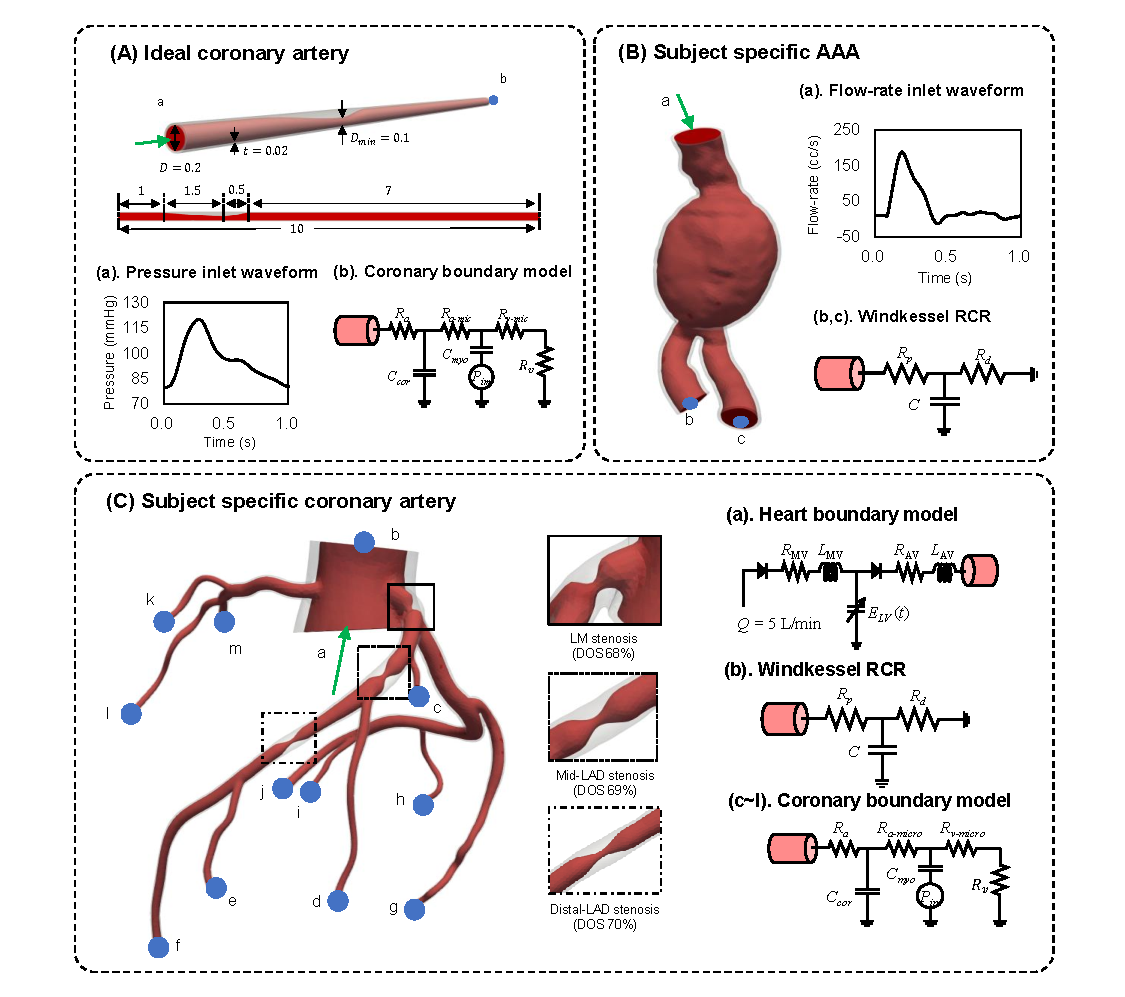
\includegraphics[width=0.95\textwidth]{figures/figure_page_02.pdf}
\caption[Idealized coronary and subject-specific AAA geometries]{(A) Idealized coronary artery geometry. (B) Subject-specific AAA geometry and boundary conditions. (C) Subject-specific coronary artery.}
\label{fig:geo_ROMFSI}
\end{figure}


\subsection{Material properties}

검증 모델의 고체·유체 물성은 문헌값을 바탕으로 부여하였다(선형탄성·고정값). 고체 물성은 Table~\ref{tab:validation-material}에 정리한다.

\begin{table}[ht]
\caption[Validation material properties]{Validation material properties (검증 모델).}
\label{tab:validation-material}
\begin{center}
\begin{tabular}{lllll}
\hline\hline
Target & $E$ & $\nu$ & $\rho$ & reference \\
\hline
Coronary wall & $1.0\times10^{7}$ dyn/cm$^2$ & 0.45 & 1.1 g/cm$^3$ & \cite{cheng1993, hsu2014, chen2021ldl, jiang2022} \\
AAA wall & $6.0\times10^{7}$ dyn/cm$^2$ & 0.49 & 1.0 g/cm$^3$ & \cite{joldes2016, figueroa2006} \\
\hline\hline
\end{tabular}
\end{center}
\end{table}

유체도메인인 혈액은 뉴턴유체 가정에 1.06 g/cm$^3$, $\mu=0.04$ poise 으로 설정하였다~\cite{fluid_newtonian_blood}

\subsection{Boundary conditions}
각 geometry의 유체 경계조건은 Figure~\ref{fig:geo_ROMFSI}와 같이 선행 연구를 참고하여 부여하였다. 이상적 LAD 관상동맥(A)에는 평균 성인 남성의 맥동 입구 압력 파형(120/80~mmHg)과 출구 lumped-parameter 관상동맥 경계조건을 부여하였다~\cite{average_pressure, coronaryBC}. 환자 특이 AAA(B)에는 MRI로 측정한 시간에 따른 유량 파형을 입구에, Windkessel RCR 모델을 출구에 부여하였다~\cite{AAA_flowrate, AAA_RCR}. 환자 특이 관상동맥(C)에는 선행 연구를 참고하여 heart inlet 및 coronary outlet 경계조건을 부여하였으며, aorta outlet(b)에만 Windkessel RCR을 설정하였다. 모든 파라미터 값은 A·B는 Table~\ref{tab:bc-ideal-aaa}에, C는 Table~\ref{tab:bc-heart-aorta} 및 Table~\ref{tab:bc-subject-coronary}에 정리한다. 

\begin{table}[ht]
\caption[Ideal coronary and AAA boundary conditions]{Ideal coronary \& AAA boundary-condition coefficients.}
\label{tab:bc-ideal-aaa}
\begin{center}
\begin{tabular}{lllr}
\hline\hline
Model & Parameter & Value & Unit \\
\hline
Ideal coronary & $R_a$ & 78827 & dyn$\cdot$s/cm$^5$ \\
(outlet b) & $C_a$ & $0.396\times10^{-6}$ & cm$^5$/dyn \\
& $R_{a\text{-micro}}$ & 128094 & dyn$\cdot$s/cm$^5$ \\
& $C_{im}$ & $3.20\times10^{-5}$ & cm$^5$/dyn \\
& $R_v$ & 19706 & dyn$\cdot$s/cm$^5$ \\
& $R_{v\text{-micro}}$ & 19706 & dyn$\cdot$s/cm$^5$ \\
& inlet & prescribed pressure (70--130 mmHg) & --- \\
AAA & $R_p$ & 450.0 & dyn$\cdot$s/cm$^5$ \\
(outlets b, c) & $C$ & $5.0\times10^{-4}$ & cm$^5$/dyn \\
& $R_d$ & 6820.0 & dyn$\cdot$s/cm$^5$ \\
& inlet & prescribed flow-rate waveform & --- \\
\hline\hline
\end{tabular}
\end{center}
\end{table}

\begin{table}[ht]
\caption[Subject-specific coronary inlet and aortic outlet BC]{Subject-specific coronary: heart inlet model (a) and aortic Windkessel RCR (b) coefficients.}
\label{tab:bc-heart-aorta}
\begin{center}
\begin{tabular}{lllr}
\hline\hline
Model & Parameter & Value & Unit \\
\hline
Heart inlet (a) & $CO$        & 5.0    & L/min \\
                & $t_{cycle}$ & 1.0    & s \\
                & $t_{sys}$   & 0.33   & s \\
                & $R_{LA}$    & 5.0    & --- \\
                & $L_{LA}$    & 1.0    & --- \\
                & $R_{LV}$    & 10.0   & --- \\
                & $L_{LV}$    & 10.0   & --- \\
                & $E_{max}$   & 2.0    & mmHg/cc \\
Aortic Windkessel RCR (b) & $R_p$ & 232.44              & dyn$\cdot$s/cm$^5$ \\
                          & $C$   & $1.50\times10^{-3}$ & cm$^5$/dyn \\
                          & $R_d$ & 1317.18             & dyn$\cdot$s/cm$^5$ \\
\hline\hline
\end{tabular}
\end{center}
\end{table}

\begin{table}[ht]
\caption[Subject-specific coronary boundary conditions]{Subject-specific coronary outlets (c--m). Units: $R$ in dyn$\cdot$s/cm$^5$; $C$ in cm$^5$/dyn.}
\label{tab:bc-subject-coronary}
\begin{center}
\small
\begin{tabular}{lrrrll}
\hline\hline
Outlet & $R_a$ & $R_{a\text{-micro}}$ & $R_{v\text{-micro}}$ & $C_a$ & $C_{im}$ \\
\hline
c & 76680 & 128624 & 39576 & $2.86\times10^{-7}$ & $2.31\times10^{-6}$ \\
d & 67588 & 113374 & 34884 & $3.97\times10^{-7}$ & $3.21\times10^{-6}$ \\
e & 65168 & 109315 & 33635 & $4.37\times10^{-7}$ & $3.53\times10^{-6}$ \\
f & 56556 & 94868  & 29190 & $6.31\times10^{-7}$ & $5.11\times10^{-6}$ \\
g & 64918 & 108895 & 33506 & $4.41\times10^{-7}$ & $3.57\times10^{-6}$ \\
h & 70224 & 117796 & 36244 & $3.60\times10^{-7}$ & $2.91\times10^{-6}$ \\
i & 71302 & 119603 & 36801 & $3.45\times10^{-7}$ & $2.79\times10^{-6}$ \\
j & 46302 & 77668  & 23898 & $1.06\times10^{-6}$ & $8.60\times10^{-6}$ \\
k & 66831 & 112104 & 34493 & $7.50\times10^{-7}$ & $6.07\times10^{-6}$ \\
l & 65058 & 109130 & 33578 & $8.04\times10^{-7}$ & $6.51\times10^{-6}$ \\
m & 55847 & 93680  & 28824 & $1.20\times10^{-7}$ & $9.70\times10^{-7}$ \\
\hline\hline
\end{tabular}
\end{center}
\end{table}

\subsection{Computational details}
모든 3차원 해석(정적 유체, prestressing, 맥동 강체벽 유체, 완전 연성 FSI)은 svFSI~\cite{zhu2022svfsi}로 수행하였고, 1D ROM 해석은 in-house C++ 솔버로 수행하였다. 3차원 해석은 Intel Xeon 프로세서(2 소켓, 96 코어)와 257~GB RAM을 갖춘 HPC 클러스터에서, 1D ROM은 Intel Core i7-12700K(3.61~GHz)·64~GB RAM 데스크톱에서 수행하였다. 혈관벽의 prestress를 얻기 위해, 수렴된 맥동 해로부터 cycle-averaged 입구 압력과 출구 유량을 계산하여 정적 유체 해석에 적용하고, 그 결과의 시간평균 벽면 traction을 구조 도메인에 prestressing 해석으로 부과하였다. 이렇게 얻은 prestress 값은 완전 연성 FSI와 제안 기법의 고체 해석에 동일하게 적용하였다~\cite{prestress}. 

\section{Validation results}

\subsection{Validation metric}
응력장 비교를 위해 심장주기 내 5개 대표 시점을 정의하였다: t_1이완기말, t_2벽운동 유발 체적변화율 최대, t_3첨두 수축기, t_4체적변화율 최소, t_5중기 이완기. 이상적 LAD 모델에서는 가속 구간이 체적변화율 극값과 일치하지 않아 추가 시점 t^*를 포함하였다.
제안 기법의 정확도는 완전 연성(ALE) 과도 3D FSI 해를 ground truth로 삼아, 동일 고체 메시 상에서 절점별로 von Mises 응력을 비교하여 정량화하였다. 각 목표 시점 t_a에서 전역 상대 L_2-노름 오차를 다음과 같이 정의한다.

\begin{equation}
e_{L2}(t_a) = \frac{\left[\sum_{i=1}^{N}\left(\sigma^{Prop}_{vm,i}(t_a) - \sigma^{FSI}_{vm,i}(t_a)\right)^2\right]^{1/2}}{\left[\sum_{i=1}^{N}\left(\sigma^{FSI}_{vm,i}(t_a)\right)^2\right]^{1/2}}
\end{equation}

여기서 $N$은 전체 고체 절점 수이다.

\subsection{Results}

% (Fig 3 --- von Mises stress contour at t_2, t_3, t_4: 세 geometry proposed vs reference FSI vs absolute error.)
\begin{figure}[ht]
\centering
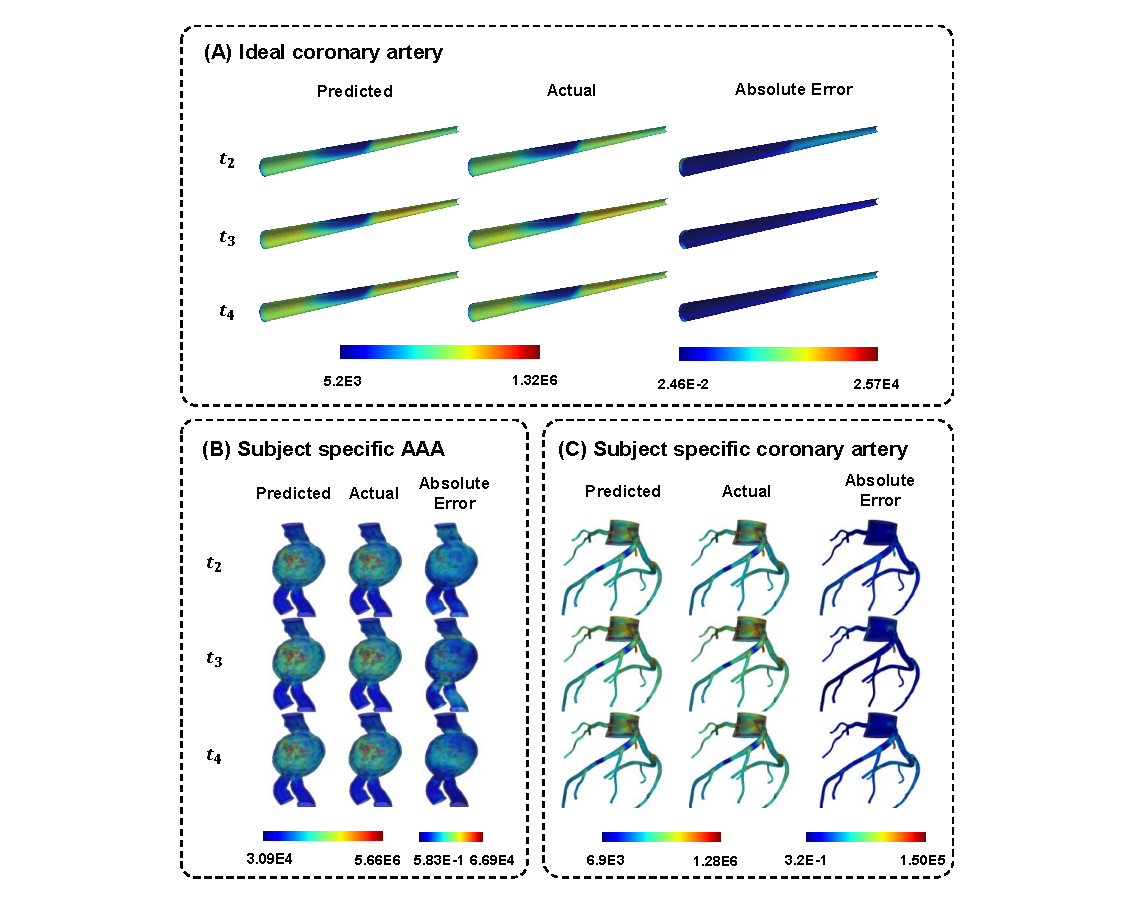
\includegraphics[width=0.95\textwidth]{figures/figure_page_03.pdf}
\caption[Validation results]{Three different geometries von Mises stress contour on each method, full FSI and snapshot-based FSI.}
\label{fig:ch2_validation}
\end{figure}

세 geometry 모두에서 제안 기법은 기준 FSI의 von Mises 응력장을 낮은 전역 상대 L_2오차로 재현하였다(Table~\ref{tab:val-l2-error}). 구체적으로 오차는 이상적 관상동맥에서 1% 미만, 환자 특이 관상동맥에서 5% 미만, AAA에서 2% 미만에 머물렀다. 시점별로는 이완기말과 중기 이완기에서 오차가 가장 작았고, 급격한 벽 운동이 일어나는 시점에서 상대적으로 커지는 경향을 보였는데, 이는 강체벽 근사가 compliant FSI 응답에서 가장 크게 벗어나는 구간이기 때문이다.
계산 비용 측면에서 제안 기법은 완전 연성 3D FSI 대비평균 220배 이상의 절감을 달성하였다(Table~\ref{tab:val-cost}). 이는 완전 맥동 3D 해석을 1D 축소차수 혈류 해석과 정적 3D snapshot 해석의 결합으로 대체한 데 따른 것이다. 한편 ramped-flow 단계는 ROM 계수 식별을 위한 geometry당 1회 전처리로, 이후 추가 snapshot 평가에서는 반복되지 않는다.
종합하면, 검증 결과는 제안 기법이 완전 과도 FSI를 정확도 손실 없이 대체하여 Chapter~3의 대규모 민감도 분석에 활용될 수 있음을 뒷받침한다.

\begin{table}[ht]
\caption[L2 error of von Mises stress]{Selected time instants and global relative $L_2$-norm error of von Mises stress.}
\label{tab:val-l2-error}
\begin{center}
\begin{tabular}{lcccccc}
\hline\hline
& \multicolumn{2}{c}{Idealized coronary} & \multicolumn{2}{c}{Subject-specific coronary} & \multicolumn{2}{c}{Subject-specific AAA} \\
Time point & Time (s) & Error (\%) & Time (s) & Error (\%) & Time (s) & Error (\%) \\
\hline
$t_1$: End-diastole & 0.05 & 0.13 & 0.05 & 1.98 & 0.08 & 0.22 \\
$t_2$: Max vol.-change & 0.15 & 0.96 & 0.15 & 3.04 & 0.15 & 1.12 \\
$t_3$: Peak systole & 0.28 & 0.28 & 0.25 & 3.91 & 0.25 & 1.00 \\
$t_4$: Min vol.-change & 0.35 & 0.91 & 0.35 & 4.45 & 0.35 & 0.87 \\
$t_5$: Mid-diastole & 0.80 & 0.15 & 0.70 & 1.62 & 0.70 & 0.30 \\
$t^{*}$: Additional & 0.45 & 0.17 & --- & --- & --- & --- \\
\hline\hline
\end{tabular}
\end{center}
\end{table}

\begin{table}[ht]
\caption[Computational time]{Computational time (min).}
\label{tab:val-cost}
\begin{center}
\begin{tabular}{lrrr}
\hline\hline
Simulation stage & Idealized coronary & Subject-specific coronary & Subject-specific AAA \\
\hline
Ramped-flow$^{a}$ & 3.3 & 33 & 5 \\
1D pulsatile & 0.2 & 3 & 0.9 \\
3D steady fluid & 1.2 & 15 & 7 \\
3D steady solid & 8 & 65 & 21 \\
\textbf{Total (proposed)} & \textbf{12} & \textbf{116} & \textbf{34} \\
Full 3D FSI & 6866 & 9989 & 1030 \\
\hline\hline
\end{tabular}\\
$^{a}$ geometry당 1회 전처리 단계.
\end{center}
\end{table}



%%======================================================================
%% Chapter 3. Parametric Analysis Framework
%%======================================================================
\chapter{Parametric Analysis Framework for Plaque Rupture Risk}

% (Fig --- Workflow overview: 3 stages: (1) dataset generation, (2) VI selection, (3) surrogate-based global sensitivity analysis.)

본 장에서는 관상동맥 플라크의 파열 위험을 형태학적·혈류역학적·재료적 인자에 대해 체계적으로 규명하기 위한 \textbf{3단계 파라메트릭 분석 프레임워크}를 제시한다. 분석은 (1) Chapter~2에서 검증한 비용효율적 맥동성 FSI를 forward solver로 사용하여, 플라크 종류별(LAP 1{,}000 / CP 1{,}300) 입출력 데이터셋을 생성하고(Stage~1), (2) 응력과 강도의 비로 정의되는 파열 취약성 지표(vulnerability index, VI) 후보를 형성한 뒤 임상 기준에 적합한 지표들을 선별하며(Stage~2), (3) 선정된 VI에 대해 가우시안 과정 회귀(Gaussian process regression, GPR) 대리모델을 학습하고, 소볼(Sobol) 분산 기반 전역 민감도 분석으로 각 인자군의 기여도를 정량화하는 순서로 진행된다.

\section{Data generation (Stage 1)}

비용효율 FSI를 이용해 두 가지 플라크 표현형(phenotype)에 대한 입출력 데이터셋을 각각 구축하였다. 대상은 \textbf{이상화된 관상동맥 모델}이며, 표현형은 서로 다른 구성거동을 보존하기 위해 분리하여 모델링하였다:

\begin{itemize}
\item \textbf{LAP (low-attenuation plaque)}: 혈관벽, 섬유막(fibrous cap, FC), 지질핵(lipid core)의 \textbf{3개 고체 도메인}.
\item \textbf{CP (calcified plaque)}: 위 3개에 석회화(calcification) 도메인을 더한 \textbf{4개 고체 도메인}.
\end{itemize}

기본(고정) 형상은 원통형 관상동맥 분절로, 길이 $10$~cm, 내강 반경 $r_\mathrm{ref}=0.1$~cm, 벽 두께 $t_\mathrm{wall}=0.02$~cm로 고정하였다.

형태학적 입력 변수는 비침습적이고 범용성이 높은 관상동맥 CT 혈관조영(CCTA)에서 도출하는 것을 전제로 하여, 향후 임상 적용으로의 확장이 용이하도록 설계하였다. 다만 섬유막 두께는 CCTA로 분해되지 않고 OCT 등 침습 영상으로만 측정 가능하므로, 공간적으로 균일하다고 가정하여 단일 스칼라로 환원하고 모든 샘플에서 $t_\mathrm{FC}=100\ \mu\mathrm{m}$로 고정하였다. 이 값은 파열 취약 플라크의 in vivo OCT 측정과 부합한다~\cite{ref12, ref13}. 이로써 침습 영상이 필요한 유일한 형태 변수를 제거하여, 전체 입력공간을 CCTA만으로 구성할 수 있는 단독 워크플로우와의 정합성을 유지한다.

% (Fig 3 --- Idealized coronary model geometry + morphological parameters.)

\subsection{Input parameters}

입력 변수는 \textbf{형태학적·혈류역학적·재료적} 세 인자군으로 구성되며, 변수별 기호·단위·범위는 Table~\ref{tab:input-vars}에 정리한다.

\begin{itemize}
\item \textbf{형태학적(morphological) 변수}
\begin{itemize}
\item 협착도 $DS$ [\%]: 최소내강 지름 기준 협착률, $DS=(1-r_\mathrm{min}/r_\mathrm{ref})\times100$.
\item 병변 길이 $L_\mathrm{lesion}$ [cm].
\item 내강 축방향 왜도 $\gamma_z$: 병변 중점 대비 최소내강면적(MLA) 위치의 정규화 축방향 편이.
\item 양성 재형성 지수 $PI$: 병변부와 기준부의 내강 단면적 비.
\item 지질핵 호 각도 $\theta_\mathrm{lipid}$ [$^\circ$]: 최대 지질부담 단면에서의 원주방향 각도 범위.
\item 지질 길이비 $r_\mathrm{lipid}=L_\mathrm{lipid}/L_\mathrm{lesion}$.
\item (CP 전용) 석회화 분율 $f_\mathrm{calc}$: lipid core 부피 대비 석회화 부피 분율.
\end{itemize}
\item \textbf{혈류역학적(hemodynamic) 변수}: 수축기압 $P_\mathrm{sys}$, 맥압 $\Delta P=P_\mathrm{sys}-P_\mathrm{dia}$, 이완기 감쇠비 $\tau$. LHS 시 $P_\mathrm{dia}>40$~mmHg 제약을 부과.
\item \textbf{재료적(material) 변수}: $E_\mathrm{vessel}$, $E_\mathrm{FC}$, $E_\mathrm{lipid}$, (CP 전용) $E_\mathrm{calc}$의 영률(CGS 단위). 관상동맥은 심장주기 동안 작은 변형 영역에서 거동하므로 모든 조직을 \textbf{선형탄성·등방성}으로 가정.
\end{itemize}

입력공간은 \textbf{라틴 하이퍼큐브 샘플링(LHS)}으로 채웠다. LAP는 12개 변수에 대해 1{,}000개 입력벡터를, CP는 18개 변수에 대해 1{,}300개 입력벡터를 추출하였다. CP의 18개는 14개 분석 입력에 석회화 생성 파라미터 4개를 더한 것이며, 별도 Sobol 분석에서 기여가 무시할 수준으로 확인되어 \textbf{최종 민감도 분석에서는 제외하고 $f_\mathrm{calc}$·$E_\mathrm{calc}$만 포함한 14개}를 입력으로 정의하였다.

\begin{table}[ht]
\caption[Input variables]{Input variables, symbols, units, and sampling ranges.}
\label{tab:input-vars}
\begin{center}
\small
\begin{tabular}{llllr}
\hline\hline
Group & Variable & Symbol & Unit & Range [min, max] \\
\hline
Morphological & Degree of stenosis & $DS$ & \% & [25, 75] \\
& Lesion length & $L_\mathrm{lesion}$ & cm & [1.0, 3.0] \\
& Lumen axial skewness & $\gamma_z$ & --- & [$-0.5$, $0.5$] \\
& Positive remodeling index & $PI$ & --- & [0.9, 1.2] \\
& Lipid arc angle & $\theta_\mathrm{lipid}$ & $^\circ$ & [120, 270] \\
& Lipid length ratio & $r_\mathrm{lipid}$ & --- & [0.5, 0.8] \\
& Calcified fraction (CP) & $f_\mathrm{calc}$ & --- & [0.10, 0.80] \\
Hemodynamic & Systolic pressure & $P_\mathrm{sys}$ & mmHg & [100, 170] \\
& Pulse pressure & $\Delta P$ & mmHg & [35, 80] \\
& Decay ratio & $\tau$ & --- & [0.01, 0.50] \\
Material & Vessel-wall modulus & $E_\mathrm{vessel}$ & dyn/cm$^2$ & [$1\times10^6$, $1.4\times10^7$] \\
& Fibrous-cap modulus & $E_\mathrm{FC}$ & dyn/cm$^2$ & [$4\times10^6$, $2.3\times10^7$] \\
& Lipid-core modulus & $E_\mathrm{lipid}$ & dyn/cm$^2$ & [$1\times10^4$, $1\times10^6$] \\
& Calcification modulus (CP) & $E_\mathrm{calc}$ & dyn/cm$^2$ & [$7\times10^9$, $2.5\times10^{11}$] \\
\hline\hline
\end{tabular}
\end{center}
\end{table}

\subsection{Geometry construction and meshing}

각 LHS 샘플마다 Autodesk Inventor로 파라메트릭 CAD 모델을 프로그래밍 방식으로 생성하고, 유체·고체 유한요소 메시로 분리 이산화하였다.

\textbf{석회화 형상 생성(CP 전용).} 석회화는 lipid core 내부에서 \textbf{seed 기반 region-growing 알고리즘}으로 생성하여 불규칙한 임상적 형태를 재현하였다(전 과정은 Appendix~A).

\begin{itemize}
\item \textbf{고체 도메인}: 병변 부근 box-meshing 전략의 \textbf{2차 사면체} 요소, 샘플당 약 $3$--$4\times10^6$개.
\item \textbf{유체 도메인}: \textbf{1차 사면체} 요소 약 $5.5\times10^6$개, 내강벽 \textbf{3겹 프리즘 경계층}.
\end{itemize}

메시 독립성은 병변 영역 대표 요소 크기를 $0.05$, $0.04$, $0.03$~cm로 변화시키며 확인하였고, $0.04$~cm와 $0.03$~cm가 사실상 동일(상대 변화 $<1\%$)하여 \textbf{$0.04$~cm}를 채택하였다.

\subsection{Boundary conditions}

% (Fig 4 --- Boundary conditions: fluid + solid)

\textbf{유체 경계조건.} 입구에는 생리학적 압력파형 $P_\mathrm{in}(t)$를 부과한다. 고정된 관상동맥 유입파형 $Q(t)$에 3-요소 Windkessel(RCR) 모델~\cite{westerhof2009windkessel}을 적합하되, 관상동맥 비 $R_p/R_d=1/10$을 고정하고 나머지 파라미터를 least-squares로 적합하였다. 입구 파형은 세 혈류역학 변수 $P_\mathrm{sys}$, $\Delta P$, $\tau$로 \textbf{완전히 결정}된다(Appendix~B). 각 출구에는 \textbf{관상동맥 미세혈관 경계조건}을 부과하였다~\cite{kim2010coronary, vignonclementel2006}.

\textbf{고체 경계조건.} Chapter~2의 정식화와 일관되게, 3D CFD에서 복원한 벽면 압력장을 다중도메인 고체 메시의 \textbf{내벽}에 surface traction으로 부과한다. 혈관 분절 양 끝단은 \textbf{고정단}으로 구속한다.

\subsection{Output parameters}

각 LHS 샘플에 대해 비용효율 FSI를 수축기 정점($t_\mathrm{sys}$)과 이완기말($t_\mathrm{dia}$) 2회 호출하여 두 시점의 응력장을 얻고, \textbf{각 노드에서 최대 주응력 $\sigma$}를 산출하였다. 이로부터 두 응력 지표를 노드별로 정의한다:

\begin{itemize}
\item \textbf{PSS} $=\sigma(t_\mathrm{sys})$: 수축기 최대 주응력 --- 단조 파단 시나리오.
\item \textbf{$\Delta$PSS} $=\sigma(t_\mathrm{sys})-\sigma(t_\mathrm{dia})$: 맥동 응력 진폭 --- \textbf{피로 파괴 시나리오}.
\end{itemize}

두 지표는 섬유막 노드 전체에서 계산하며, 단일노드 노이즈를 줄이기 위해 최대하중 노드 중심의 반경 $r=0.01$~cm 구면 이웃에서 공간 평균한다.

\section{Vulnerability Index formulation and selection (Stage 2)}

파열은 응력이 강도를 초과할 때 발생하므로, 취약성 지표를 \textbf{응력과 강도의 비}로 정의한다: $\mathrm{VI}=\mathrm{stress}/\mathrm{strength}$~\cite{corti_review}.

\subsection{VI formulation}

응력은 PSS·$\Delta$PSS 2종을 사용한다. 한편 섬유막 강도를 직접 모델링·정량화한 선행연구는 없어, 세 가지 파열 시나리오 --- (i) 고정 극한응력, (ii) 에너지밀도, (iii) 고정 극한변형률 --- 를 선형탄성 가정과 결합하여 강도를 단일 지수 $\alpha$로 매개화하였다:

\begin{equation}
\mathrm{strength} \propto E_\mathrm{FC}^{\alpha}, \qquad \alpha \in \{0.0,\ 0.5,\ 1.0\}
\end{equation}

각 지수는 고전 파괴이론에 대응한다: $\alpha=0$ Rankine(최대응력), $\alpha=0.5$ Beltrami(에너지밀도), $\alpha=1$ St.~Venant(최대변형률).

응력 2종과 강도 지수 3종을 조합하여 \textbf{6개 VI 후보}를 정의한다:

\begin{equation}
\mathrm{VI}(\sigma,\alpha) = \frac{\sigma}{E_\mathrm{FC}^{\alpha}}, \quad \sigma\in\{\mathrm{PSS},\Delta\mathrm{PSS}\},\ \alpha\in\{0.0,0.5,1.0\}
\end{equation}

각 케이스에서 섬유막 전 노드에 대해 VI를 계산하고, 그 \textbf{최댓값을 해당 케이스의 대표 VI}로 사용한다.

\subsection{VI candidate selection (seven-criterion rubric)}

6개 후보 VI를 임상적으로 확립된 고위험 플라크 특징 \textbf{7가지 기준}(Table~\ref{tab:seven-criteria})으로 선별하였다. 각 기준은 케이스별로 추출한 \textbf{플라크 feature}와 VI가 가져야 할 상관 방향을 임상 근거로부터 \emph{a priori}로 고정한 것이다. 각 (후보, 기준) 쌍에 대해 해당 feature와 VI의 \textbf{Spearman 순위상관 부호}를 계산하여, 기대 방향과 일치하면 compliant(\checkmark), 아니면 $\times$로 분류하였다. \textbf{7개 기준을 모두 만족하는 후보만 물리적으로 admissible}로 본다.

기준 7(섬유막 두께)은 본 시뮬레이션에서 $t_\mathrm{FC}$를 고정하였으므로, 나머지 입력을 평균값에 고정하고 $t_\mathrm{FC}$와 $E_\mathrm{FC}$만 변화시킨 \textbf{별도 15개 시뮬레이션}으로 평가하였다.

\begin{table}[ht]
\caption[Seven high-risk plaque features]{Seven established high-risk plaque features used for VI selection.}
\label{tab:seven-criteria}
\begin{center}
\begin{tabular}{cllc}
\hline\hline
\# & Clinical fact & Model feature & Data \\
\hline
1 & Soft plaque substrate & Low $E_\mathrm{lipid}$ & LAP \\
2 & Less calcified plaque (CP) & Low $f_\mathrm{calc}$ & CP \\
3 & Large lipid arc angle & Large $\theta_\mathrm{lipid}$ & LAP \\
4 & Large plaque burden & High lipid-core volume & LAP \\
5 & Functional gradient & High $\Delta$FFR & LAP \\
6 & Collagen-deficient fibrous cap & Low $E_\mathrm{FC}$ & LAP \\
7 & Thin fibrous cap & Low fibrous-cap thickness & * \\
\hline\hline
\end{tabular}\\
*: additional 15-sim data.
\end{center}
\end{table}

\section{Surrogate-based global sensitivity analysis (Stage 3)}

소볼 민감도 분석은 표현형당 1만 회 이상의 모델 평가를 요구하여 비용효율 FSI로도 직접 수행할 수 없다. 따라서 본 stage는 먼저 입력$\to$VI 사상을 학습하는 GPR 대리모델을 구축하고, 그 surrogate 위에서 소볼 분산 기반 전역 민감도 분석을 수행한다.

\subsection{GPR surrogate model}

각 VI 후보·표현형마다 입력벡터($d=12$ LAP, $d=14$ CP)를 스칼라 VI로 사상하는 \textbf{GPR 대리모델}을 개별 학습하였다. 유효 샘플은 \textbf{LAP 784/1{,}000, CP 1{,}075/1{,}300}이었다.

모델은 scikit-learn \texttt{GaussianProcessRegressor}로 구현하고, \textbf{ARD(Automatic Relevance Determination)} 적용 제곱지수 커널을 사용하였다. 커널 하이퍼파라미터는 주변 로그우도 최대화로 결정하였다. 정확도는 leave-one-out 교차검증 결정계수($R^2_\mathrm{LOO}$)로 보고하며, 두 표현형 모두 $R^2_\mathrm{LOO}>0.94$의 높은 예측 정확도를 보였다.

\subsection{Sobol variance-based indices}

학습된 GPR에 대해 \textbf{소볼 분산 기반 전역 민감도 분석}을 수행하였다. 입력 $X_i$의 \textbf{1차 지수}

\begin{equation}
S_i = \frac{\mathrm{Var}_{X_i}\!\left[\mathbb{E}_{X_{\sim i}}(Y\mid X_i)\right]}{\mathrm{Var}(Y)}
\end{equation}

는 $X_i$ 단독 기여를, \textbf{전차 지수}

\begin{equation}
S_{Ti} = \frac{\mathbb{E}_{X_{\sim i}}\!\left[\mathrm{Var}_{X_i}(Y\mid X_{\sim i})\right]}{\mathrm{Var}(Y)}
\end{equation}

는 상호작용을 포함한 총기여를 정량화한다. Saltelli 준난수 표본추출로 1·전차 지수를 추정하였고, 표현형당 기저표본 $N=1{,}024$로 LAP는 $14{,}336$, CP는 $16{,}384$회 surrogate 평가를 수행하였다.

개별 변수 지수에 더해, 세 인자군 $G\in\{\mathrm{형태, 재료, 혈류역학}\}$의 \textbf{군 단위 Sobol 지수}를 계산하였다:

\begin{equation}
S_G = \frac{\mathrm{Var}_{X_G}\!\left[\mathbb{E}_{X_{\sim G}}(Y\mid X_G)\right]}{\mathrm{Var}(Y)}, \qquad S_{TG} = \frac{\mathbb{E}_{X_{\sim G}}\!\left[\mathrm{Var}_{X_G}(Y\mid X_{\sim G})\right]}{\mathrm{Var}(Y)}.
\end{equation}

군 지수는 개별 지수의 단순 합이 아니라 \textbf{군 내 변수 간 상호작용까지 올바르게 반영}한다.


%%======================================================================
%% Chapter 4. Results
%%======================================================================
\chapter{Results}

본 장에서는 세 단계 프레임워크의 결과를 LAP와 CP 두 표현형에 대해 제시한다. 먼저 6개 취약성 지수 후보를 임상 기준으로 선별하여 두 개의 최종 지수를 확정하고(\S4.1), 이 지수에 대한 Sobol 전역 민감도 분석 결과를 제시하며(\S4.2), 마지막으로 파열 위치 분포 결과를 임상 데이터와 비교한다(\S4.3).

\section{취약성 지수(Vulnerability Index) 선정}

취약성 지수는 응력과 강도의 비 $\mathrm{VI} = \sigma/\mathrm{strength}$로 정의하였다. 응력 2종(PSS, $\Delta$PSS)과 강도 지수 3종($\mathrm{strength}\sim E_\mathrm{FC}^{\alpha}$, $\alpha = 0.0/0.5/1.0$)을 조합해 \textbf{6개 후보}를 만들고, 각 후보를 임상적으로 확립된 \textbf{7개 고위험 플라크 특징}에 대해 feature--VI 상관의 \emph{부호}가 임상 기대 방향과 일치하는지로 선별하였다(7개 모두 일치해야 admissible).

% (Fig 4.1 --- Input-VI correlation scatter plots.)

각 (feature, VI 후보) 쌍의 상관(Pearson $r$·Spearman $\rho$)을 산점도로 분석한 결과, row~4--7은 6개 후보가 모두 같은 부호를 보여 후보를 변별하지 못하는 반면, \textbf{row 1--3 (plaque burden·$\Delta$FFR·collagen-deficient cap)에서만 후보에 따라 상관 부호가 갈린다}. 각 상관의 부호를 임상 기대 방향과 대조한 요약이 Table~\ref{tab:vi-compliance}이다.

\begin{table}[ht]
\caption[VI compliance matrix]{Compliance of the six Vulnerability Index candidates with the seven high-risk plaque features. \checkmark: clinically consistent; $\times$: violates expected direction.}
\label{tab:vi-compliance}
\begin{center}
\small
\begin{tabular}{clcccccc}
\hline\hline
\# & High-risk feature & PSS / $E^{0.0}$ & PSS / $E^{0.5}$ & PSS / $E^{1.0}$ & $\Delta$PSS / $E^{0.0}$ & $\Delta$PSS / $E^{0.5}$ & $\Delta$PSS / $E^{1.0}$ \\
\hline
1 & Large plaque burden & $\times$ & $\times$ & $\times$ & \checkmark & \checkmark & \checkmark \\
2 & High $\Delta$FFR & $\times$ & $\times$ & $\times$ & \checkmark & \checkmark & \checkmark \\
3 & Collagen-deficient cap & $\times$ & \checkmark & \checkmark & $\times$ & \checkmark & \checkmark \\
4 & Soft plaque & \checkmark & \checkmark & \checkmark & \checkmark & \checkmark & \checkmark \\
5 & Large lipid arc angle & \checkmark & \checkmark & \checkmark & \checkmark & \checkmark & \checkmark \\
6 & Less calcified plaque & \checkmark & \checkmark & \checkmark & \checkmark & \checkmark & \checkmark \\
7 & Thin fibrous cap & \checkmark & \checkmark & \checkmark & \checkmark & \checkmark & \checkmark \\
\hline
& \textbf{All 7 satisfied?} & $\times$ & $\times$ & $\times$ & $\times$ & \textbf{\checkmark} & \textbf{\checkmark} \\
\hline\hline
\end{tabular}
\end{center}
\end{table}

6개 후보 중 \textbf{$\Delta$PSS$/E_\mathrm{FC}^{0.5}$와 $\Delta$PSS$/E_\mathrm{FC}^{1.0}$ 두 열만 7기준을 모두 만족}하며, VI1, VI2로 표기한다. 탈락 양상은 두 가지다.

\begin{itemize}
\item \textbf{PSS 후보($\alpha$ 무관)} --- plaque burden·$\Delta$FFR에서 VI가 음의 상관($\rho \approx -0.1$)을 보여 ``부담·$\Delta$FFR 증가 $\to$ 위험 증가''와 어긋난다. 같은 두 feature에서 $\Delta$PSS는 양의 상관($\rho \approx +0.1$--$+0.2$)으로 부호를 회복한다 $\to$ \textbf{피로 진폭 $\Delta$PSS가 필요}.
\item \textbf{$\alpha=0.0$ 후보(강도 정규화 없음)} --- collagen-deficient cap에서 VI--$E_\mathrm{FC}$가 양의 상관($\rho \approx +0.43$)이 되어 ``$E_\mathrm{FC}$ 감소 $\to$ 위험 증가''를 위배한다. $\alpha\geq 0.5$로 $E_\mathrm{FC}$를 분모에 넣으면 음의 상관($\rho \approx -0.35$--$-0.79$)으로 뒤집힌다 $\to$ \textbf{$\alpha > 0$(재료 정규화)이 필요}.
\end{itemize}

따라서 응력 = $\Delta$PSS, 강도 = $E_\mathrm{FC}^{\alpha}$($\alpha > 0$)일 때에만 7기준을 동시에 충족하며, VI1·VI2를 최종 지수로 채택한다.

\section{민감도 분석 결과}

\subsection{GPR 대리모델 정확도}

확정된 두 지수(VI1, VI2)에 대해, 각 표현형의 입력$\to$VI 사상을 학습하는 GPR 대리모델을 구축하였다. 학습에 사용한 유효 입출력 쌍과 정확도는 다음과 같다: LAP 784/1{,}000, $R^2_\mathrm{LOO}=0.9598$(VI1); CP 1{,}075/1{,}300, $R^2_\mathrm{LOO}>0.93$.

\subsection{Sobol 전역 민감도 지수}

% (Fig 4.2 --- Sobol sensitivity (A) individual (B) group)

GPR 대리모델 위에서 Saltelli 샘플링으로 1차 지수($S_1$)와 전차수 지수($S_T$)를 산출하였다. \textbf{개별 민감도}에서 지배 인자는 VI1·VI2 모두에서 \textbf{재료 모듈러스($E_\mathrm{vessel}$, $E_\mathrm{FC}$)와 수축기압($P_\mathrm{sys}$)}이다. \textbf{그룹 민감도}에서 두 표현형(LAP·CP)·두 지수(VI1·VI2) 모두에서 \textbf{재료물성군(Material)이 지배적}이었으며, 그 다음으로 혈류역학적 인자군이 높은 민감도를 보였다. 형태학적 인자군은 개별 1차 지수는 낮지만 전차 지수가 상대적으로 큰 것으로 확인된다.

\section{파열 위치 결과}

% (Fig 4.3 --- Rupture location (A) circumferential (B) axial)

파열 위치 지수로부터 얻은 파열 위치 분포를 원주방향과 축방향으로 나누어 분석하였다. 파열 위치는 한 case 내에서 가장 높은 VI의 위치이므로, PSS와 $\Delta$PSS에 따른 두 그룹으로 구분된다.

원주방향에서는 \textbf{shoulder}에서의 파열이 PSS·$\Delta$PSS 각각 \textbf{56.9\%, 57.5\%}로 더 빈번하게 발생하는 것으로 확인된다. 축방향에서는 \textbf{minimum lumen area} 앞뒤 영역인 middle 영역에서 \textbf{60.2\%, 67.3\%}로 더 빈번하게 파열이 발생하는 것으로 확인된다.


%%======================================================================
%% Chapter 5. Discussion
%%======================================================================
\chapter{Discussion}

\section{맥동성-인지 응력: $\Delta$PSS 대 PSS}

\S4.1의 취약성 지수 선정 결과는 맥동성이 기계적으로 중요하다는 가설을 정량적으로 직접 뒷받침한다. 검토된 6개 VI 후보 중 임상적으로 허용 가능한 모든 후보는 단조 최대 수축기 응력(PSS)이 아닌 맥동 응력 진폭 $\Delta$PSS를 기반으로 구성되어 있었다. 기계학적으로 이는 플라크 파열을 피로(fatigue)형 거동으로 해석하는 관점과 일치한다. 즉, 섬유막은 단일 임계값 초과 하중에 의해 한순간에 파괴되는 것이 아니라 매 심박 주기마다 손상이 누적되며, 그 누적의 지배적 구동력은 주기 응력의 진폭이다. 동일한 해석은 Bank 등~\cite{bank_fatigue_hypothesis}이 단일 임계 사건이 아닌 고주기·저진폭 반복 하중이 섬유막 파괴를 지배한다고 가설로 제안한 바 있고, 이후 Versluis 등~\cite{versluis_paris_fatigue}이 Paris 법칙 기반의 피로 균열 성장 모델로 전산적으로 입증한 바와 같다. 보다 최근에는 Costopoulos 등~\cite{costopoulos_vh_ivus}이 관상동맥 in vivo VH-IVUS 코호트에서 파열된 fibroatheroma가 비파열 병변보다 유의하게 큰 수축기--이완기 응력 진폭($\Delta$PSS)을 보임을 보고하고(55 vs.\ 43~kPa, $p=0.02$), 이 주기적 신장--이완 하중을 명시적으로 ``plaque fatigue''의 구동력으로 제시하였다. 본 연구의 결과는 임상적으로 확립된 7개 파열-위험 특징에 걸친 임상-일관성 필터 하에서 물리적으로 허용 가능한 모든 VI가 $\Delta$PSS 기반 형태로 귀결됨을 보임으로써 이 증거 체계를 확장한다. 이는 in-silico 취약성 평가의 기본선으로서 정상 상태가 아닌 맥동성 혈류역학의 채택을 정당화한다.

\section{강도 정규화의 필요성: $\alpha > 0$의 임상적 정합성}

호환성 매트릭스는 또한 두 $\alpha=0$ 후보가 섬유막 강성 기준(Table~\ref{tab:seven-criteria}, Fact~1)을 만족하지 못했음을 보여준다. 생물학적 근거는 다음과 같다. 섬유막 탄성계수는 독립적인 기계적 조절 변수가 아니라 콜라겐 함량의 직접적 대리지표이다. Savvopoulos 등~\cite{savvopoulos_collagen_modulus}은 인간 관상동맥 플라크 조직에서 국소 영률과 콜라겐 섬유 함량 사이에 유의한 양의 상관($\rho=0.53$, $p=0.036$)을 보고하였고, 콜라겐이 풍부한 cap 영역이 빈약한 영역보다 현저히 강성이 높음을 확인하였다($p<0.001$). Chai 등~\cite{chai_indentation}은 인간 경동맥 플라크에 대한 압입 시험에서 동일한 경향을 입증하였다. 이를 콜라겐 감소가 cap을 약화시키고 파열 위험을 높인다는 임상 관찰과 결합하면 ``$E_\mathrm{FC}$가 클수록 $\Leftrightarrow$ 콜라겐 풍부 $\Leftrightarrow$ 파열 위험 감소''의 인과 사슬이 성립한다.

이 관계는 입력--출력 상관 결과에서도 정량적으로 확인된다. $\alpha=0$의 경우 $E_\mathrm{FC}$가 증가할수록 VI가 오히려 증가하여 cap이 강성화될수록 위험이 커지는 --- 조직학과 정반대인 --- 관계가 나타난다. Rankine 형의 순수-응력 기준($\alpha=0$)이 이 의존성을 제거한 직접적 결과이다. 응력 분자를 $\alpha>0$인 $E_\mathrm{FC}^\alpha$ 형태의 강도 분모와 결합하면, 콜라겐이 풍부하고 강성이 높은 cap이 갖는 조직 강도 이득까지 함께 부호화되어 임상적으로 기대되는 방향이 회복된다.

$\alpha$의 크기 자체도 의미를 갖는다. 민감도 분석 결과에서 $\alpha=0.5$와 $1.0$ 사이의 상위 3개 인자 순위는 동일하지만, $\alpha$가 커질수록 재료 인자군의 1차 지수 합이 단조 증가한다. 구체적으로, 재료 인자군의 1차 지수 합은 LAP에서 $\alpha=0.5$일 때 0.602에서 $\alpha=1.0$일 때 0.797로, CP에서 0.626에서 0.836으로 증가한다 --- 두 표현형 모두에서 $\alpha$를 0.5에서 1.0으로 강화하면 재료 인자군이 설명하는 출력 분산 비중이 약 20~\%p 상승한다. 본 연구에서는 강도를 $E_\mathrm{FC}$의 거듭제곱으로 단순화하였으나, 이는 강도가 본질적으로 재료 물성의 함수임을 반영한 추상화이며, $\alpha$-의존적 민감도 변화는 결국 강도라는 양 자체가 재료 물성에 의해 좌우됨을 정량적으로 드러낸다.

\section{재료-지배적 민감도 위계}

\S4.2에서 확립된 인자군 순위는 임상적 위험 층화에 직접적인 시사점을 갖는다. VI 분산에 기여하는 두 최대 개별 인자인 $E_\mathrm{vessel}$과 $E_\mathrm{FC}$는 모두 재료 물성이며, 통합된 중요도 위계에서도 재료 및 혈류역학 인자가 취약성의 지배적 구동 인자로 자리한다. 재료 물성은 국소 응력--강도 균형을 직접 결정하고, 맥동성 혈류역학은 섬유막이 견뎌야 하는 주기 하중의 크기를 결정한다. 두 인자군은 함께 두 VI 정의와 두 표현형 모두에서 1차 출력 분산의 대부분을 설명한다.

이와 대조적으로 형태학적 변수들은 1차 지수 $S_i$가 현저히 작은 반면 총-차수 지수 $S_{Ti}$는 두드러지게 크게 나타났다. 정량적으로, 형태학적 인자군의 총-차수와 1차의 차이($S_T - S_1$)는 LAP에서 $0.283 - 0.151 = 0.132$, CP에서 $0.244 - 0.151 = 0.093$로 나타나, 형태학 영향의 절반 이상이 상호작용 항을 통해 발현됨을 보인다. 이는 기계학적으로 자연스러운 결과이다. 주어진 lipid arc, plaque burden, 양성 재형성 지수는 그 자체로는 파열-관련 응력 집중을 결정하지 못하고, 기저의 cap·혈관벽 강성 및 맥압과 컨볼루션될 때 비로소 의미를 가진다. 따라서 결론은 형태학이 중요하지 않다는 것이 아니라, 그 예후 가치가 동시 측정된 재료·혈류역학 상태에 조건부라는 것이다. 다수의 영상 기반 점수처럼 형태학적 기술자를 독립적 위험 표지자로 취급하는 방식은 결과적으로 상호작용 항이 부호화하는 상당한 분산을 폐기하는 셈이며, 이는 형태학적 고위험 특징의 단독 예측력이 제한적이라는 임상 관찰과도 일치한다.

\section{한계}

본 연구의 세 가지 한계를 명시한다.

첫째, 본 연구는 이상화된 기하 가정을 채택하였다. 구체적으로 축대칭성을 가정하였고, 섬유막 두께를 공간적으로 균일하다고 보았으며, 혈관 축방향 굴곡(tortuosity)·측지·분기를 배제하였다. 이는 1{,}000 샘플 규모의 매개변수 민감도 분석을 수행 가능하게 만들기 위한 형상 생성 단계의 단순화로, 형상 매개변수 공간을 통제 가능한 차원으로 축소하기 위한 조치이다. 향후 환자-특이적 CT/OCT 영상에서 재구성된 비대칭·비균일·굴곡을 포함한 기하를 입력으로 사용할 경우, 본 연구에서 확립된 $\Delta$PSS 기반 VI 및 재료-지배 위계 결론의 환자 단위 적용성을 직접 검증할 수 있을 것이다.

둘째, 구성 모델로 선형탄성을 채택하였다. 이는 주기적 관상동맥 변형이 일반적으로 미소-변형 영역에 머문다는 점에서 정당화되며, GPR 대리모델 학습에 필요한 1{,}000회 규모의 반복 FSI 해석을 비용효율적으로 수행하기 위한 선택이다. 다만 파열-임박 cap 주변에서는 국소 변형이 비선형 영역으로 진입할 수 있으므로, 추후 Holzapfel--Gasser--Ogden 형태~\cite{hgo} 등의 초탄성·비등방 기술과 lipid pool·섬유막·석회화 inclusion의 구성요소-분해 표현을 결합한 모델로의 확장이 우선순위 높은 후속 과제로 남는다.

셋째, 섬유막 강도는 $E_\mathrm{FC}$의 거듭제곱 형태로 단순화되었다. 이는 강도의 환자-특이적 직접 측정이 현재 임상 영상 모달리티로는 불가능하다는 제약 하에서, 강도를 재료 물성의 함수로 모델링한 추상화이다. 향후 micro-indentation, atomic force microscopy, 또는 영상 기반 강성--강도 상관 모델 등을 통해 환자별 강도 값의 직접 측정이 가능해진다면, 본 거듭제곱 가정을 측정값으로 대체하여 VI를 환자-특이적으로 평가할 수 있을 것이다.


%%======================================================================
%% Chapter 6. Concluding Remark
%%======================================================================
\chapter{Concluding Remark}

본 학위논문은 비용효율적 맥동성 FSI 프레임워크를 GPR 대리모델 및 Sobol 전역 민감도 분석과 결합하여, 관상동맥 플라크 파열의 형태학적·혈류역학적·재료적 결정 인자를 두 표현형(LAP 1{,}000 / CP 1{,}300 샘플)·맥동 조건 하에서 \textbf{동시에} 정량화하였다. 두 가지 주요 발견은 다음과 같다.

첫째, 임상적으로 확립된 7개 고위험 플라크 특징을 모두 만족하는 취약성 지표는 \textbf{맥동 응력 진폭($\Delta$PSS)을 응력으로 사용하고 섬유막 강도 정규화 $\alpha>0$을 갖는 두 지수에 한정}되었다. 이는 플라크 파열을 피로(fatigue) 누적 거동으로 해석하는 관점과, 강도가 본질적으로 재료 물성의 함수임을 동시에 지지한다.

둘째, 인자군 단위 Sobol 분석에서 \textbf{재료물성군이 두 표현형·두 지수 모두에서 지배 인자군}이며, $\alpha$ 강화에 따라 그 비중이 LAP $0.602 \to 0.797$, CP $0.626 \to 0.836$으로 단조 증가하였다. 개별 지배 인자는 $E_\mathrm{vessel}$, $E_\mathrm{FC}$, $P_\mathrm{sys}$였고, 형태학적 변수는 1차 지수보다 전차 지수가 크게 나타나 그 영향이 주로 재료·혈류역학과의 상호작용을 통해 발현됨이 확인되었다.

종합하면, 본 학위논문은 in-silico 플라크 파열 평가의 baseline으로서 맥동성 혈류역학과 강도 정규화의 채택을 정당화하고, 임상 변환의 우선축이 형태학적 영상 계측 단독이 아닌 \textbf{환자-특이적 조직 강성 특성화}에 있음을 제시한다. 향후 환자-특이적 기하·비선형 구성모델·직접 측정 강도값을 통합한 확장 연구가 본 프레임워크의 임상 적용성을 한층 강화할 것으로 기대된다.


%%======================================================================
%% Bibliography (placeholder — to be replaced by references.bib import)
%%======================================================================
\begin{thebibliography}{99}

\bibitem{who_cvd_burden} World Health Organization, \textit{Cardiovascular diseases (CVDs) fact sheet}, 2021.
\bibitem{libby_pathophysiology} P. Libby, \textit{Mechanisms of acute coronary syndromes and their implications for therapy}, NEJM, 2013.
\bibitem{virmani_vulnerable_plaque} R. Virmani et al., \textit{Pathology of the vulnerable plaque}, JACC, 2006.
\bibitem{cardoso_plaque_mechanics} L. Cardoso, S. Weinbaum, \textit{Microcalcifications, their genesis, growth, and biomechanical stability in fibrous cap rupture}, 2018.
\bibitem{akyildiz_review} A. C. Akyildiz et al., \textit{Effects of intima stiffness and plaque morphology on peak cap stress}, BMC, 2011.
\bibitem{teng_pss} Z. Teng et al., \textit{Plaque structural stress (PSS) studies}, 2014.
\bibitem{huang_pss} Y. Huang et al., \textit{Computational modeling of plaque stress}, 2016.
\bibitem{savvopoulos_collagen_modulus} F. Savvopoulos et al., \textit{Local Young's modulus--collagen correlation in coronary plaque}, 2020.
\bibitem{chai_indentation} C.-K. Chai et al., \textit{Local mechanical properties of human atherosclerotic plaques}, JBM, 2014.
\bibitem{corti_review} A. Corti et al., \textit{Vulnerability index review}, 2022.
\bibitem{bank_fatigue_hypothesis} A. J. Bank et al., \textit{Cyclic loading hypothesis of plaque rupture}, 2000.
\bibitem{versluis_paris_fatigue} A. Versluis et al., \textit{Fatigue crack growth in fibrous cap}, J. Biomech., 2006.
\bibitem{costopoulos_vh_ivus} C. Costopoulos et al., \textit{$\Delta$PSS in VH-IVUS cohort}, EHJ, 2019.
\bibitem{ohayon_morpho_only} J. Ohayon et al., \textit{Morphological sensitivity}, 2008.
\bibitem{kim_snapshot} H. Kim et al., \textit{Snapshot-based cost-effective FSI framework}, under review, 2024.
\bibitem{choi2025rom} S. Choi et al., \textit{Physics-based 1D ROM with stenosis pressure drop}, 2025.
\bibitem{masson2011} I. Masson et al., \textit{Nonlinear vascular wall constitutive model}, 2011.
\bibitem{cheng1993} G. C. Cheng et al., \textit{Distribution of circumferential stress in ruptured vs. stable plaques}, Circulation, 1993.
\bibitem{hsu2014} M.-C. Hsu et al., \textit{FSI of coronary arteries}, 2014.
\bibitem{chen2021ldl} H. Chen et al., \textit{LDL-transport coronary FSI}, 2021.
\bibitem{jiang2022} Y. Jiang et al., \textit{Coronary wall modulus reference}, 2022.
\bibitem{joldes2016} G. Joldes et al., \textit{AAA wall stress model}, 2016.
\bibitem{figueroa2006} C. A. Figueroa et al., \textit{Coupled-momentum method for vascular FSI}, 2006.
\bibitem{zhu2022svfsi} S. Zhu et al., \textit{svFSI open-source solver}, 2022.
\bibitem{ref12} \textit{OCT thin-cap reference}.
\bibitem{ref13} \textit{OCT thin-cap reference}.
\bibitem{westerhof2009windkessel} N. Westerhof et al., \textit{The arterial Windkessel}, Med.\ Biol.\ Eng.\ Comput., 2009.
\bibitem{kim2010coronary} H. J. Kim et al., \textit{Patient-specific modeling of coronary blood flow}, 2010.
\bibitem{vignonclementel2006} I. E. Vignon-Clementel et al., \textit{Outflow boundary conditions for 3D simulations}, 2006.
\bibitem{hgo} G. A. Holzapfel, T. C. Gasser, R. W. Ogden, \textit{A new constitutive framework for arterial wall mechanics}, 2000.

\end{thebibliography}


%%======================================================================
%% 감사의 글
%%======================================================================
\acknowledgment[1]
[TODO: 감사의 글 작성.]


%%======================================================================
%% 약력
%%======================================================================
\curriculumvitae[1]

\begin{personaldata}
    \name       {김 세 혁}
    \dateofbirth{1999}{12}{28}
    \birthplace {대한민국}
    \address    {[TODO]}
\end{personaldata}

\begin{education}
    \item[2018. 3.\ --\ 2024. 2.] 한국과학기술원 기계공학과 (학사)
    \item[2024. 3.\ --\ 2026. 2.] 한국과학기술원 기계공학과 (석사)
\end{education}

\begin{career}
    \item[TODO] TODO
\end{career}

\begin{publication}
    \item [TODO] TODO
\end{publication}

\label{paperlastpagelabel}
\end{document}
